\chapter{Word Enrichment}

We already know a lot about our model, but wouldn’t it be great to see where it was right and were it was wrong? The \widget{Confusion Matrix} widget can do exactly that!\marginnote{To observe a particular misclassification, click on a cell in the matrix.\\
\\
To output all the misclassified documents, use 'Select Misclassified'. This will output selected documents for further inspection.}

The matrix has correctly predicted documents in the diagonal (blue) and incorrectly predicted documents in off-diagonal (red). We can see that no Animal Tales were wrongly predicted as Tales of Magic, but 4 Tales of Magic were incorrectly predicted as Animal Tales.

\vspace{-0.2cm}
\begin{figure*}[h]
  \centering
  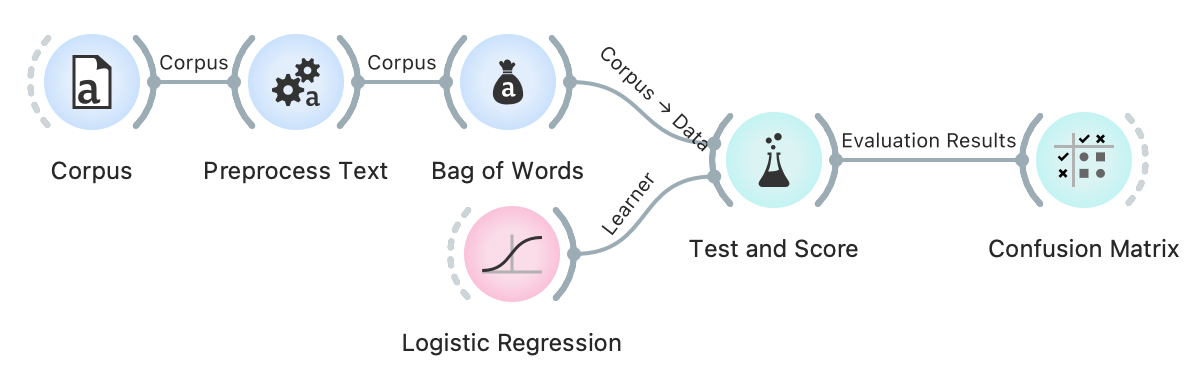
\includegraphics[width=0.8\linewidth]{workflow.png}%
  \caption{$\;$}
\end{figure*}
\vspace{-0.3cm}

\vspace{-0.2cm}
\begin{figure*}[h]
  \centering
  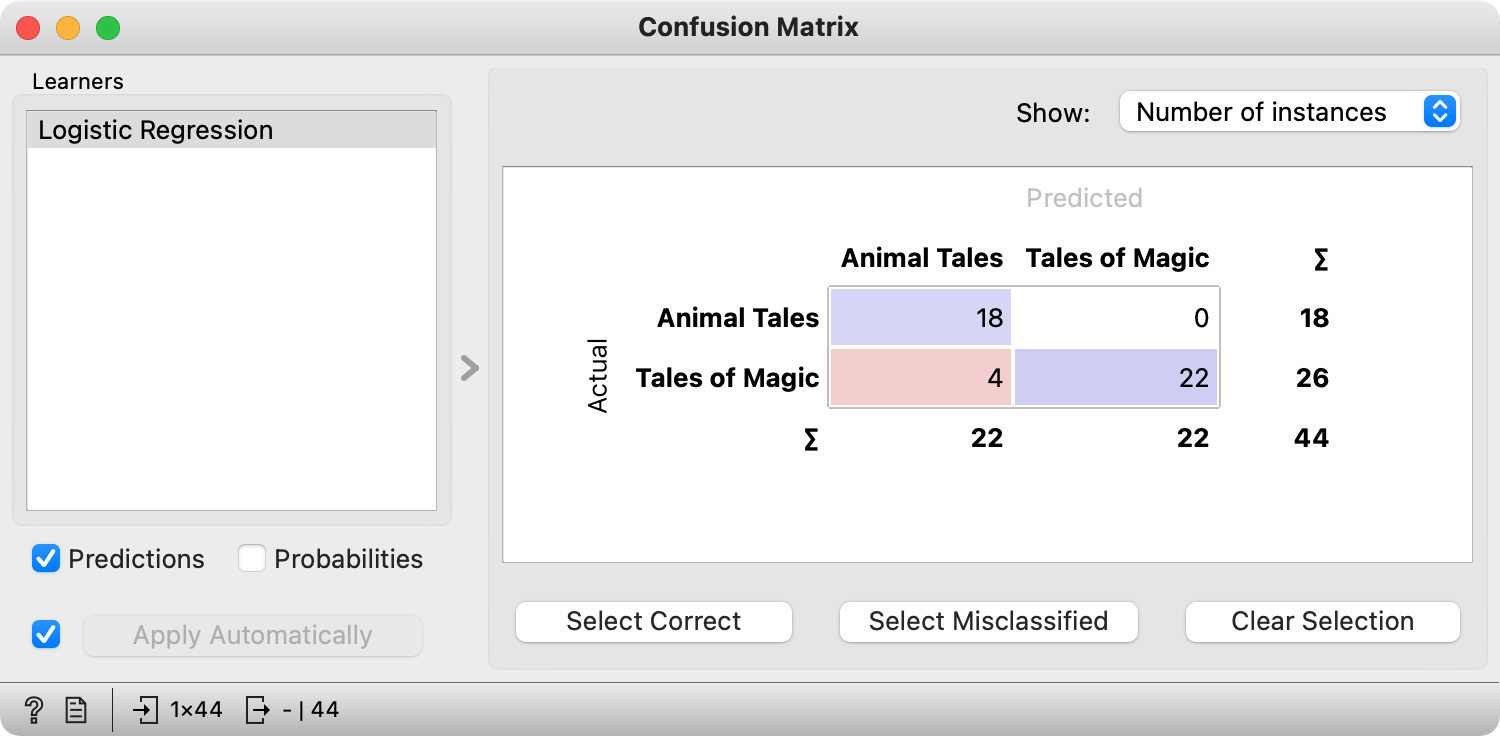
\includegraphics[width=0.8\linewidth]{confusion-matrix.png}%
  \caption{$\;$}
\end{figure*}
\vspace{-0.3cm}

But why? What is so different about these documents, that the model failed to predict the right class?

We can reuse \widget{Corpus Viewer} to inspect the misclassified documents. Or even better, observe which words are significant in each subset!

\newpage
\clearpage

Word Enrichment compares a subset of documents against the entire corpus and finds statistically significant words for the selected subset.

\vspace{-0.2cm}
\begin{figure*}[h]
  \centering
  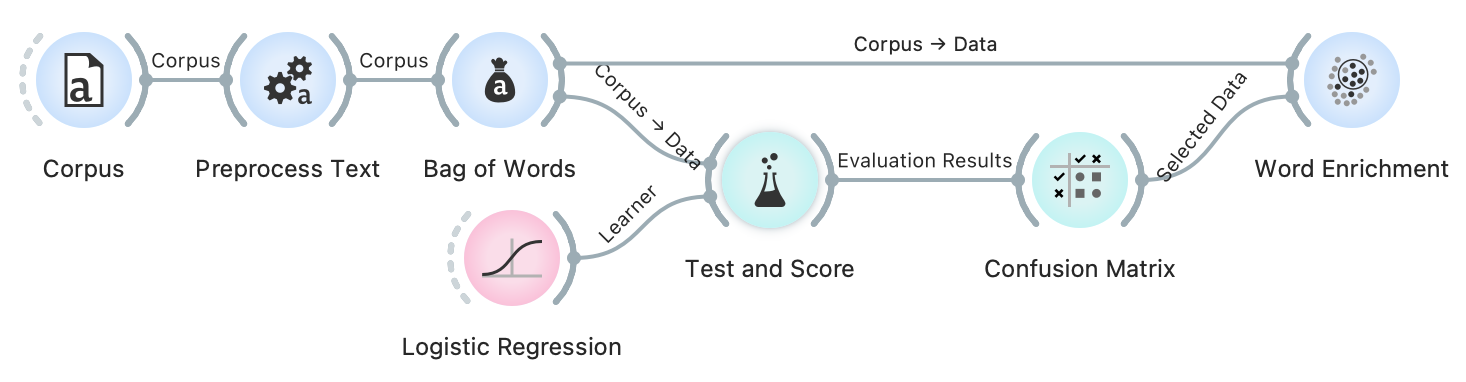
\includegraphics[width=\linewidth]{workflow2.png}%
  \caption{$\;$}
\end{figure*}
\vspace{-0.3cm}

For correctly classified Animal Tales, \emph{wolf} is a significant word representing those documents.\marginnote{Word Enrichment works on any kind of subset. In Corpus Viewer, browse for documents containing the word \emph{queen}. Now pass this subset to \widget{Word Enrichment}. Don't forget to connect \widget{Bag of Words} as well - Word Enrichment needs the entire data set against which to compare the subset.} For correctly classified Tales of Magic, the list is much longer and contains words such as \emph{king}, \emph{beautiful}, \emph{man}, etc. These results are very similar to what we have observed in a Nomogram. This is indeed just a different way of inspecting the model!

So the next time you see the word \emph{wolf} in a text, you can bet the text is an animal tale! :)

\begin{figure*}[h]
    \centering
    \infinitewidthbox{
      \stackinset{r}{-0.2\linewidth}{t}{+0.25\linewidth}
      {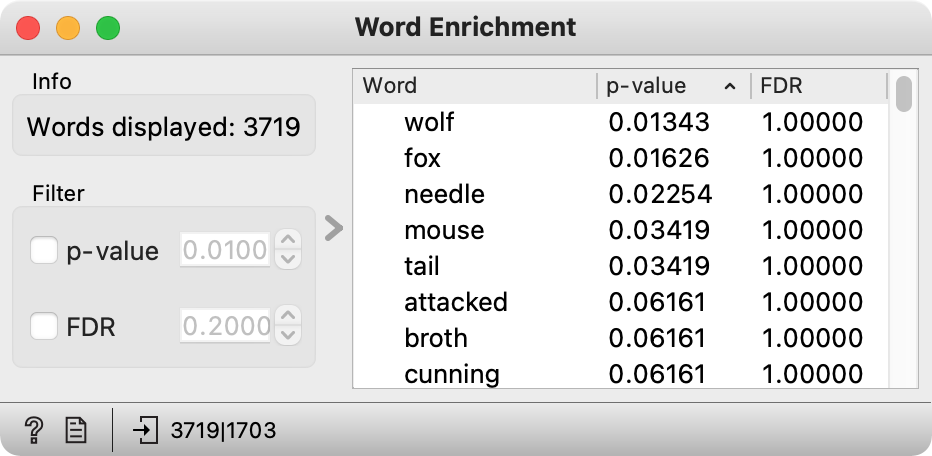
\includegraphics[scale=0.5]{word-enrichment.png}}
      {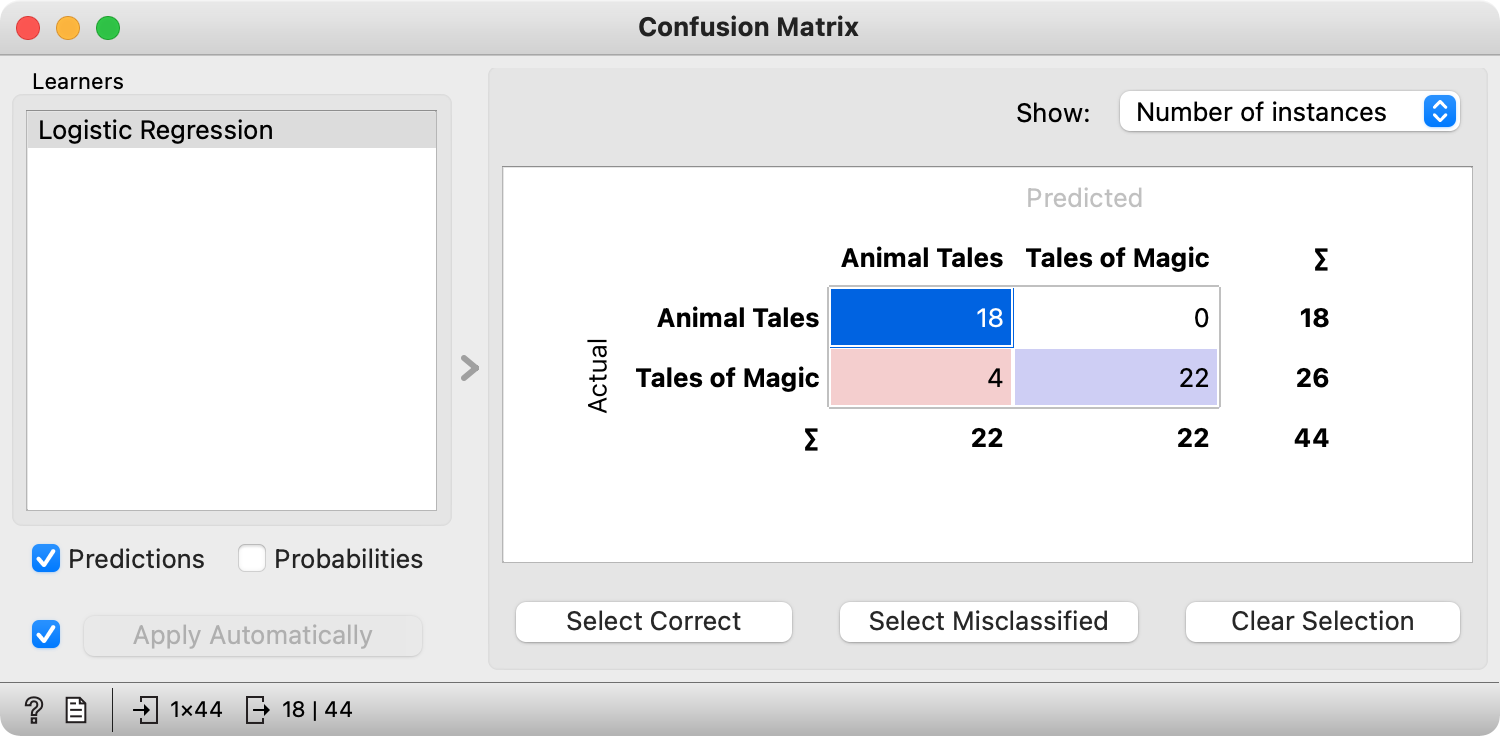
\includegraphics[scale=0.5]{confusion-matrix-selection.png}}
      \hspace{2cm}
      }
    \caption{$\;$}
\end{figure*}
